\documentclass[10pt,a4paper]{article}
\usepackage{float}
\usepackage{graphicx}

\title{Digital signal processing}
\author{Lucas Swartsenburg (6174388) \and Sander van Veen (6167969)}

\begin{document}

\maketitle


\newpage

\section*{Opgave 1} % {{{
\label{sec:Opgave 1}

\begin{enumerate}
    \item $ \Omega = 2\pi * f * T_s = 2\pi * 20 Hz * \frac{1}{1000} \; samples
        \; s^{-1} = 0.04 \pi  $.

    \noindent $ N = \frac{1000}{20} = 50 $.

    \[ 2 \times \frac{50 \pi}{3200} < \frac{128 \pi}{3200} < 3 \times
    \frac{50 \pi}{3200} \]

    \noindent Dus tussen de tweede en derde harmonische trilling.

    \item $ \Omega = 2\pi * f * T_s = 2\pi * 30 Hz * \frac{1}{1000} \; samples
        \; s^{-1} = 0.06 \pi  $.

    \noindent $ N = \frac{1000}{30} = 33 \frac{1}{3} $.

    \[ 3 \times \frac{200 \pi}{12800} < \frac{786 \pi}{12800} < 4 \times
    \frac{200 \pi}{12800} \]

    \noindent Dus tussen de derde en vierde harmonische trilling.
    De pieken vinden plaats op de harmonische trilling.\\
    \item Filled in table:
    
    \begin{tabular}{|r|l|l|l|} \hline
        f & $\Omega$ met $T_s = 0.001$  & Periode $N$ & ?de harm $< \Omega<$ ?de
        harm \\ \hline
        $20 Hz$ & $0.04\pi$ & $50$ & 2de $< \Omega <$ 3de \\ \hline 
        $30 Hz$ & $0.06\pi$ & $33\frac{1}{3}$ & 3de $< \Omega <$ 4de \\ \hline 
    \end{tabular}
    \item De pieken in de spectra zijn te vinden op de plaatsen waartussen de harmonischen te vinden zijn.

    \begin{figure}[H]
    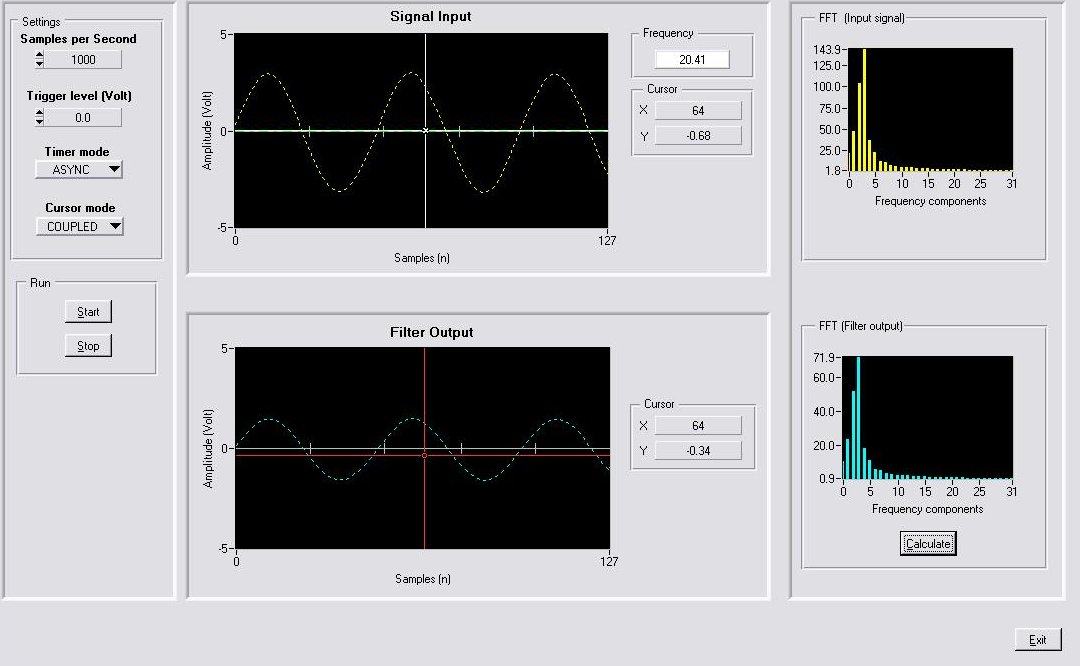
\includegraphics[scale=0.5]{1000_20.JPG}
    \caption{$f=20Hz$ $T_{s}=0.001$}
    \end{figure}
    \begin{figure}[H]
    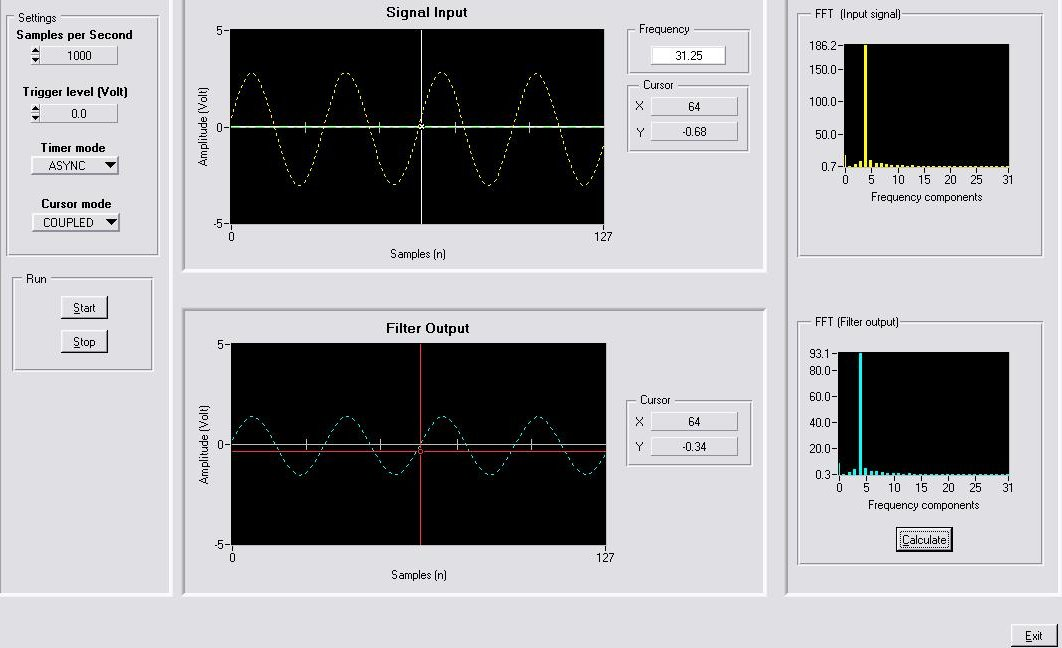
\includegraphics[scale=0.5]{1000_30.JPG}
    \caption{$f=30Hz$ $T_{s}=0.001$}
    \end{figure}


\end{enumerate}

% }}}

\section*{Opgave 2} % {{{
\label{sec:Opgave 2}

\begin{enumerate}
    \item $ \Omega = 2\pi * f * T_s = 2\pi * 20 Hz * \frac{1}{500} \; samples
        \; s^{-1} = 0.08 \pi $.

    \noindent $ N = \frac{500}{20} = 25 $.

    \[ 5 \times \frac{50 \pi}{3200} < \frac{256 \pi}{3200} < 6 \times
    \frac{50 \pi}{3200} \]

    \noindent Dus tussen de vijfde en zesde harmonische trilling.

    \item $ \Omega = 2\pi * f * T_s = 2\pi * 30 Hz * \frac{1}{500} \; samples
        \; s^{-1} = 0.12 \pi  $.

    \noindent $ N = \frac{500}{30} = 16\frac{2}{3} $.

    \[ 7 \times \frac{50 \pi}{3200} < \frac{384 \pi}{3200} < 8 \times
    \frac{50 \pi}{3200} \]

    \noindent Dus tussen de zevende en achtste harmonische trilling.
    De pieken vinden plaats op de harmonische trilling.\\

    \begin{tabular}{|r|l|l|l|} \hline
        f & $\Omega$ met $T_s = 0.001$  & Periode $N$ & ?de harm $< \Omega<$ ?de
        harm \\ \hline
        $20 Hz$ & $0.08\pi$ & $25$ & 5de $< \Omega <$ 6de \\ \hline
        $30 Hz$ & $0.12\pi$ & $16\frac{2}{3}$ & 7de $< \Omega <$ 8ste \\ \hline 
    \end{tabular}
    \item De pieken in de spectra zijn te vinden op de plaatsen waartussen de harmonischen te vinden zijn.

    \begin{figure}[H]
    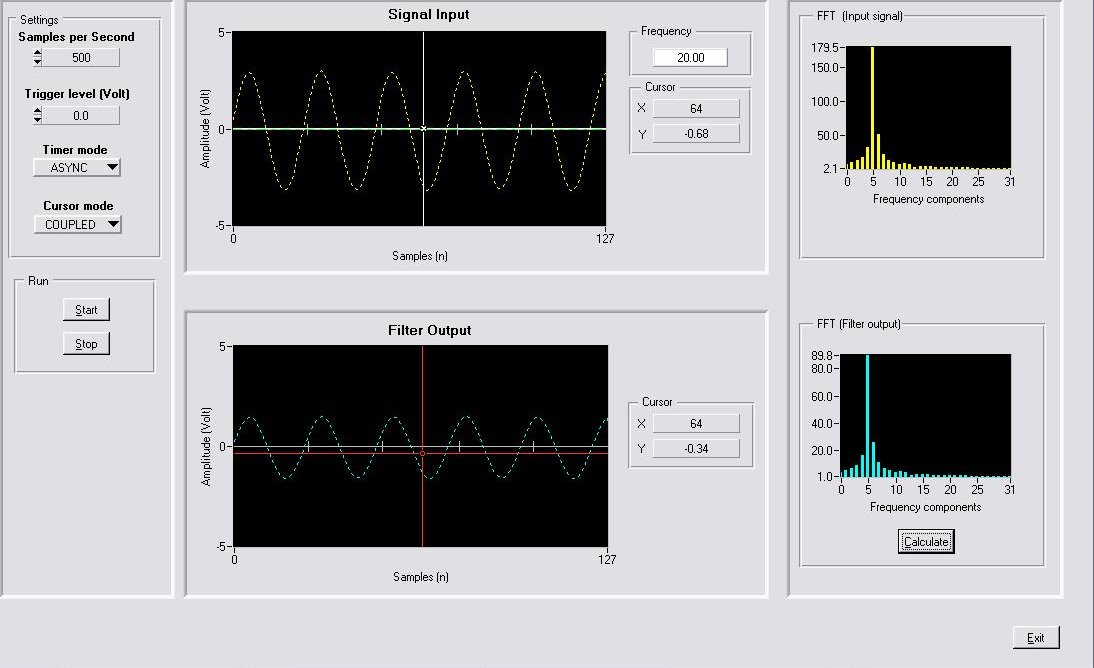
\includegraphics[scale=0.5]{500_20.JPG}
    \caption{$f=20Hz$ $T_{s}=0.002$}
    \end{figure}
    \begin{figure}[H]
    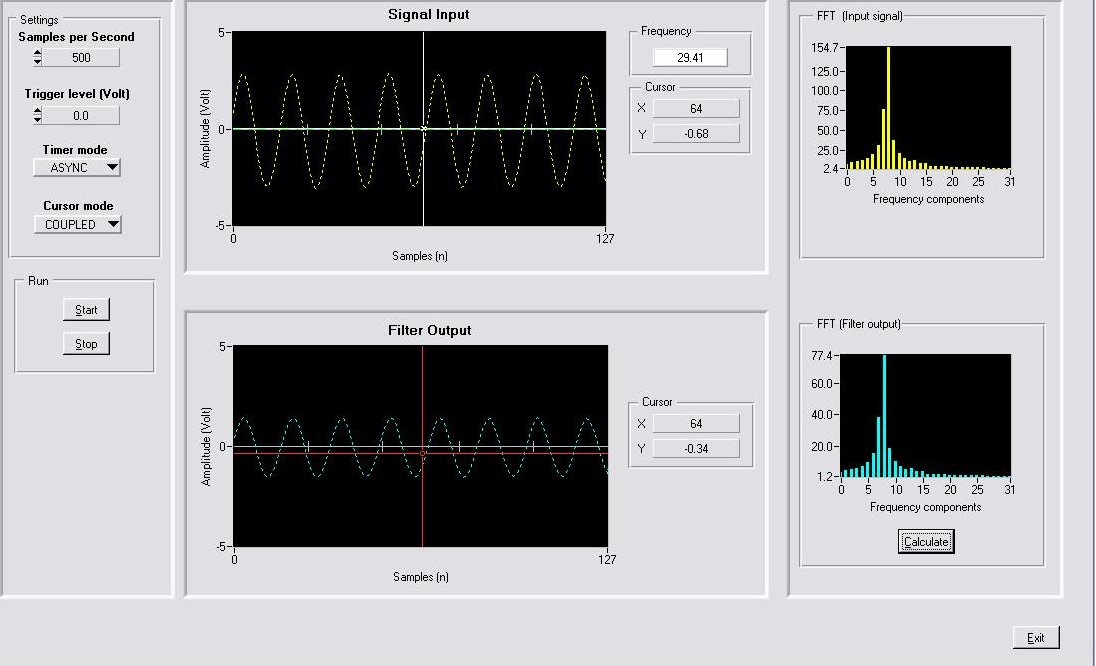
\includegraphics[scale=0.5]{500_30.JPG}
    \caption{$f=30Hz$ $T_{s}=0.002$}
    \end{figure}



\end{enumerate}

% }}}

\section*{Opdracht 3} % {{{
\label{sec:Opdracht 3}

\begin{enumerate}
    \item $ \Omega = 2\pi * f * T_s = 2\pi * 20 Hz * \frac{1}{1000} \; samples
        \; s^{-1} = 0.04 \pi $.

    \noindent $ N = \frac{1000}{20} = 50 $.

    \item Tussen de tweede en derde harmonische trilling.
    \[ 2 \times \frac{50 \pi}{3200} < \frac{128 \pi}{3200} < 3 \times
    \frac{50 \pi}{3200} \]

    \item Na de tweede en derde harmonische trilling zijn de $5n+3$-de
    trillingen ook harmonisch (met $n$ als geheel getal en $n > 0$).

    \item $H(z) = 0.5 \frac{z}{z-0.9} \rightarrow b_0 = 0.5, b_1 = 0, a_1 = 0.9$

    \item $y[n] - a_1y[n-1] = b_0x[n] + b_1x[n-1]
        \rightarrow y[n] - 0.9y[n-1] = 0.5x[n]$

    Deze differentievergelijking wordt omgezet naar de volgende C expressie:

    \begin{verbatim}
filterInput[0] = 0.5 * filterInput[n];

for(i = 1; i < arrayLength; i++) {
    filterInput[n] = 0.5 * filterInput[n] + 0.9 filterOutput[n-1];
}
    \end{verbatim}

    \item $H(1) = 0.5 \frac{1}{1 - 0.9} = 5 $

    \item Het lowpassfilter is correct.

    \begin{figure}[H]
    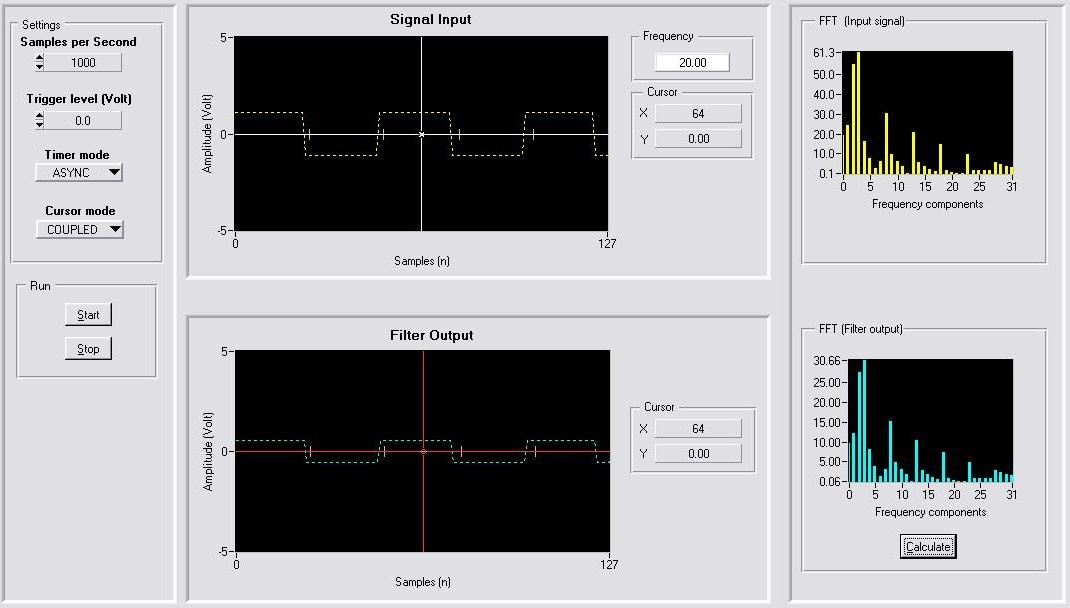
\includegraphics[scale=0.5]{blok_1000_20.JPG}
    \caption{Blok signal met $f=20Hz$ $T_{s}=0.001$}
    \end{figure}
 

\end{enumerate}

% }}}

\section*{Opgave 4} % {{{
\label{sec:Opgave 4}

\begin{enumerate}
    \item $ \Omega = 2\pi * f * T_s = 2\pi * 20 Hz * \frac{1}{1000} \; samples
        \; s^{-1} = 0.04 \pi $.

    \noindent $ N = \frac{1000}{20} = 50 $.

    \item Tussen de tweede en derde harmonische trilling.
    \[ 2 \times \frac{50 \pi}{3200} < \frac{128 \pi}{3200} < 3 \times
    \frac{50 \pi}{3200} \]

    \item Na de tweede en derde harmonische trilling zijn de $5n+3$-de
    trillingen ook harmonisch (met $n$ als geheel getal en $n > 0$).

    \item $z_0 = cos(\frac{3\pi}{64}) + j \, sin(\frac{3\pi}{64}) =
    e^{-j\frac{3\pi}{64}}$ en $z_1 =
    cos(\frac{\pi}{32}) + j \, sin(\frac{\pi}{32}) = e^{-j\frac{\pi}{32}}$.

    \item $H(z) = \frac{z}{z-0.9} \rightarrow b_0 = 1, b_1 = 0, a_1 = 0.9$

    \item We hebben de berekening in python uitgevoerd:

    \begin{verbatim}
>>> def H(z):
...     return z / (z-0.9)
...
>>> z1 = cmath.cos(cmath.pi/32) + 1j * cmath.sin(cmath.pi/32)
>>> z0 = cmath.cos(3*cmath.pi/64) + 1j * cmath.sin(3*cmath.pi/64)
>>> z0
(0.98917650996478101+0.14673047445536175j)
>>> z1
(0.99518472667219693+0.098017140329560604j)
>>> H(z0)
(3.7222743068438988-4.4792132008597303j)
>>> H(z1)
(5.5890607078154106-4.7256174714656467j)
>>> abs(H(z0))
5.8239743229298577
>>> abs(H(z1))
7.3190887467134509
    \end{verbatim}

    Hieruit volgt: $|H(z_0)| \approx 5.823974$ en $|H(z_1)| \approx 7.319089$
\end{enumerate}

    \begin{figure}[H]
    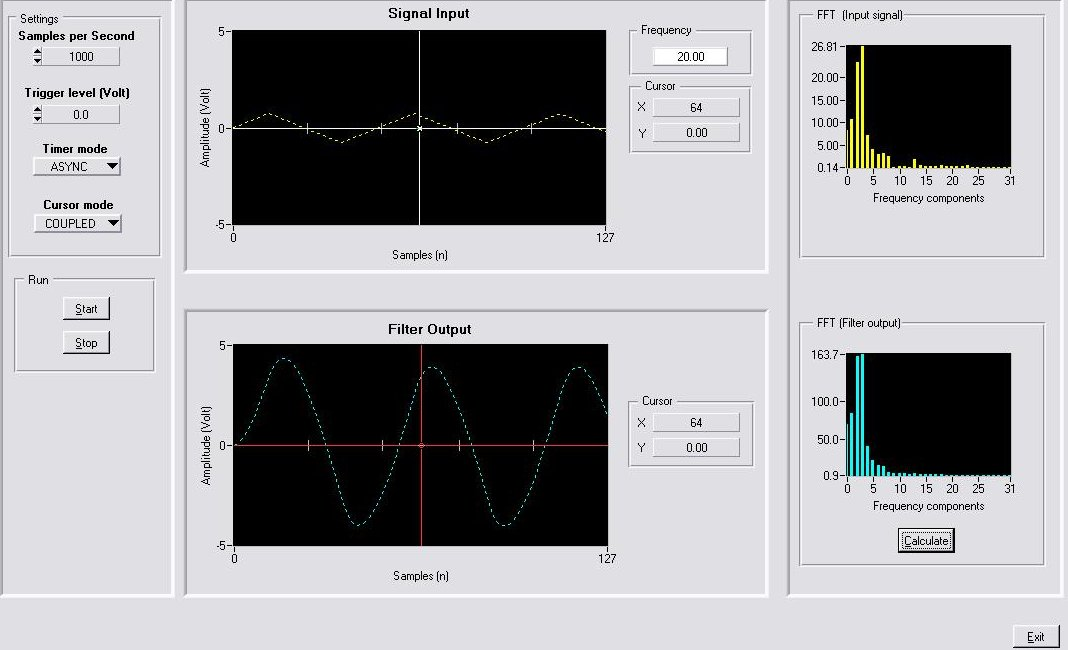
\includegraphics[scale=0.5]{ramp_filter_1000_20.JPG}
    \caption{Ramp signal met $f=20Hz$ $T_{s}=0.001$}
    \end{figure}
 
% }}}

\section*{Opgave 5} % {{{
\label{sec:Opgave 5}

\begin{enumerate}
    \item $ H(z) = K \frac{(z - z_0)(z - z_1)}{z^2}
               = \frac{z^2 - 2\, z \, cos(\pi/10) + 1}{z^2} = \frac{z^2 -
               1.902113z + 1}{z^2} $

    \noindent $ y[n] = 2cos(\pi/10)y[n-1] - y[n-2] + x[n] $

    \item De tabel ingevuld:
    \begin{table}[H] \centering
    \begin{tabular}{|l|l|l|} \hline
    f & $\Omega$ met $T_s = 0.001$ & $|H(e^{j\Omega})|$ \\ \hline
    10 Hz & $ \frac{\pi}{50}$  & 0.093940     \\ \hline
    20 Hz & $ \frac{\pi}{25}$  & 0.082116     \\ \hline
    30 Hz & $ \frac{3\pi}{50}$ & 0.062461     \\ \hline
    40 Hz & $ \frac{2\pi}{25}$ & 0.035053     \\ \hline
    50 Hz & $ \frac{\pi}{10}$  & 1.110223e-16 \\ \hline
    60 Hz & $ \frac{3\pi}{25}$ & 0.042560     \\ \hline
    \end{tabular}
    \end{table}

\item Uit onze resultaten blijkt dat het signaal bij 50hz er bijna niet meer is. We kunnen concluderen dat het filter de 50hz frequenties wegfiltert.

\end{enumerate}

% }}}

\end{document}
% vim: foldmethod=marker:
